% "Look to my coming on the first light of the fifth day, at dawn look to the east."
%   -- Gandalf

\documentclass[12pt]{caltech_thesis}
\usepackage{graphicx}
\usepackage{rotating}
\usepackage{todonotes}

\usepackage[utf8]{inputenc}
\usepackage[T1]{fontenc}
\usepackage{newtxtext, newtxmath}

\usepackage{natbib}
\usepackage[labelstoglobalaux, sectionbib]{bibunits}
\usepackage{aas_macros}
\defaultbibliographystyle{aasjournal}

\usepackage{hyperref}

\usepackage{tikz}
\usetikzlibrary{shapes, arrows, positioning, calc}

\tikzset{
    base/.style = {text width=3cm, text centered,},
    node/.style = {base, draw, minimum height=1.5cm, fill=white, semithick, scale=0.8},
    process/.style = {node, rectangle, fill=black!15},
    data/.style = {node, rectangle, rounded corners},
    line/.style = {draw, semithick, color=black!90},
    arrow/.style = {line, -to},
    arrow-dashed/.style = {arrow, dashed},
    % styles for drawing lines with 2 elbows
    -|-/.style={
        to path={
            (\tikztostart) -| ($(\tikztostart)!#1!(\tikztotarget)$) |- (\tikztotarget)
            \tikztonodes
        }
    },
    -|-/.default=0.5,
    |-|/.style={
        to path={
            (\tikztostart) |- ($(\tikztostart)!#1!(\tikztotarget)$) -| (\tikztotarget)
            \tikztonodes
        }
    },
    |-|/.default=0.5,
}

\usepackage{custom}

\begin{document}

\title{Searching for the Cosmic Dawn}
\author{Michael William Eastwood}

\degreeaward{Doctor of Philosophy in Astrophysics} % Degree to be awarded
\university{California Institute of Technology}    % Institution name
\address{Pasadena, California}                     % Institution address
\unilogo{caltech.png}                              % Institution logo
\copyyear{2019}                                    % Year (of graduation) on diploma
\defenddate{September 3, 2018}                     % Date of defense

\orcid{0000-0002-4731-6083}

\rightsstatement{Some rights reserved. This thesis is distributed under a ``Creative Commons Attribution-ShareAlike License''}

\maketitle[logo]

\begin{acknowledgements}
    This thesis would not have been possible without the support of my family and friends.

    First, and most importantly, \ty to my parents whom have always been my first port of call for
    advice and support.  \Ty to Shawn for his extraordinary patience in helping me pass my first
    physics class, and teaching me through example that math is rewarding (although I still maintain
    my assertion that math is a subfield of physics).  \Ty to Kevin for being my lifelong friend.

    \Ty to my entire thesis committee, but especially to my advisor Gregg Hallinan.

    Sebastian

    Melodie

    Jackie

    \Ty to Marin Anderson for being a wonderful friend and peer. We started on the OVRO-LWA project
    together,

    Ryan M

    \Ty to Stephen Bourke and Jake Hartman without whom the OVRO-LWA would not be the instrument it
    is today. \Ty to Harish Vedantham whose patient and thorough discussions with me were often
    extremely influential in helping me find new direction in my research.

    \Ty to the entire Owens Valley Radio Observatory staff, without whom the OVRO-LWA would not even
    exist.

    \Ty to Richard Shaw for developing the $m$-mode analysis framework that was foundational for
    this thesis, and to Adrian Liu who first introduced me to his work.

    \Ty to Gita Patel and Althea Keith for dealing with my occasional delinquency.

    \Ty to Patrick Shopbell

    \Ty to my mentor Ryan Trainor, who in spite of the fact that he is a Liverpool fan, helped me
    settle and find my feet within the Caltech community. \Ty to Jacob Jencson and Chris Bochenek

    Caltech peoples
    Yi

    Judd, Tzu-Ching, Sievers

    Maci, Eva, John

    \Ty to professors Marjorie Corcoran, Christopher Johns-Krull, Patrick Hartigan, James
    Hannon, Mark Embree, and Anthony Chan who collectively guided me through my time at Rice
    University.

    \Ty to everybody who has played on the Cataclysmics soccer team. We occasionally won a game or
    two. Maybe results will improve with the new management.

    Finally, \ty to Jessica Tran for helping me grow in my faith and praying the rosary with
    me daily.



\end{acknowledgements}

\begin{abstract}
    [This abstract must provide a succinct and informative condensation of your work. Candidates are welcome to prepare a lengthier abstract for inclusion in the dissertation, and provide a shorter one in the CaltechTHESIS record.]
\end{abstract}

\extrachapter{Published Content and Contributions}

[Fill this out with my publications]

\tableofcontents
\listoffigures
\listoftables
%\printnomenclature

\mainmatter

\chapter{Introduction}

\begin{bibunit}

The discovery of the cosmic microwave background (CMB) radiation by \citet{1965ApJ...142..419P}
provided the first direct evidence that the universe had a beginning. Arno Penzias and Robert Wilson
shared the 1978 Nobel Prize in Physics for this discovery, and astronomers have been studying this
radiation ever since. In fact, a second Nobel Prize was awarded to John Mather and George Smoot in
2006 for their work on the Cosmic Background Explorer (COBE) satellite, which was amongst the first
experiments to demonstrate that the background radiation was anisotropic
\citep{1992ApJ...396L...1S}. These studies of the CMB have fundamentally advanced humanity's
understanding of the universe: its origin, evolution, and composition. Still we continue to study
the CMB particularly because it illuminates everything in the universe. It is a flashlight for the
darkness of space within our expanding universe.

As the universe expands, the wavelength of a photon is similarly stretched or redshifted (so-called
because it gradually drifts to longer, redder wavelengths). Photons originating from a star 1000
light-years away will travel through the universe for 1000 years before they are collected by our
telescopes. Consequently we observe this star as it was 1000 years ago. However, during its travels,
the photon was also stretched by a small factor of $0.000007\%$ due to the expansion of the
universe.  For nearby stars, this expansion factor is clearly too small to be conceivably measured.
However, with the discovery of the first quasar by \citet{1963Natur.197.1040S} it soon became
apparent that the stretching factor, the redshift $z$, can be $>10\%$. Today, the most distant known
quasars and galaxies are so far away that the wavelength has more than doubled ($z > 1$) due to the
expansion of the universe \citep{2011Natur.474..616M, 2015ApJ...810L..12Z, 2016ApJ...819..129O,
2018Natur.553..473B}.

Due largely to careful and detailed work studying the CMB \citep[e.g.,][]{2016A&A...594A..25P}, Type
Ia supernova explosions \citep[e.g.,][]{1998AJ....116.1009R,1999ApJ...517..565P}, and cosmological
galaxy surveys \citep[e.g.,][]{2001MNRAS.328.1039C}, we have a coherent and consistent understanding
of the expansion history of the universe. Consequently the redshift $z$ is commonly used as a proxy
for distance. The higher the redshift, the longer the photon has been in transit, and the further
its origin.

Despite its abundance, neutral hydrogen has few low energy transitions that allow it to be traced.
Consequently astronomers resort to using a hyperfine structure transition arising from the magnetic
dipole interaction between proton and electron. This interaction leads to a slight energy difference
between the spin-symmetric state and the spin-antisymmetric state. The energy difference is $hc /
(21\,\text{cm})$ where $h$ is Planck's constant, and $c$ is the speed of light. Consequently when a
Hydrogen atom transitions from the spin-symmetric state (higher energy) to the spin-antisymmetric
state (lower energy), it emits a photon with a wavelength of $21\,\text{cm}$ or a frequency of
$1420\,\text{MHz}$. The redshift $z$ of a 21~cm photon is therefore computed from the observed
frequency $\nu$ as
\begin{equation}
    z = \frac{1420\,\text{MHz}}{\nu} - 1\,.
\end{equation}

\begin{figure}[t]
    \centering
    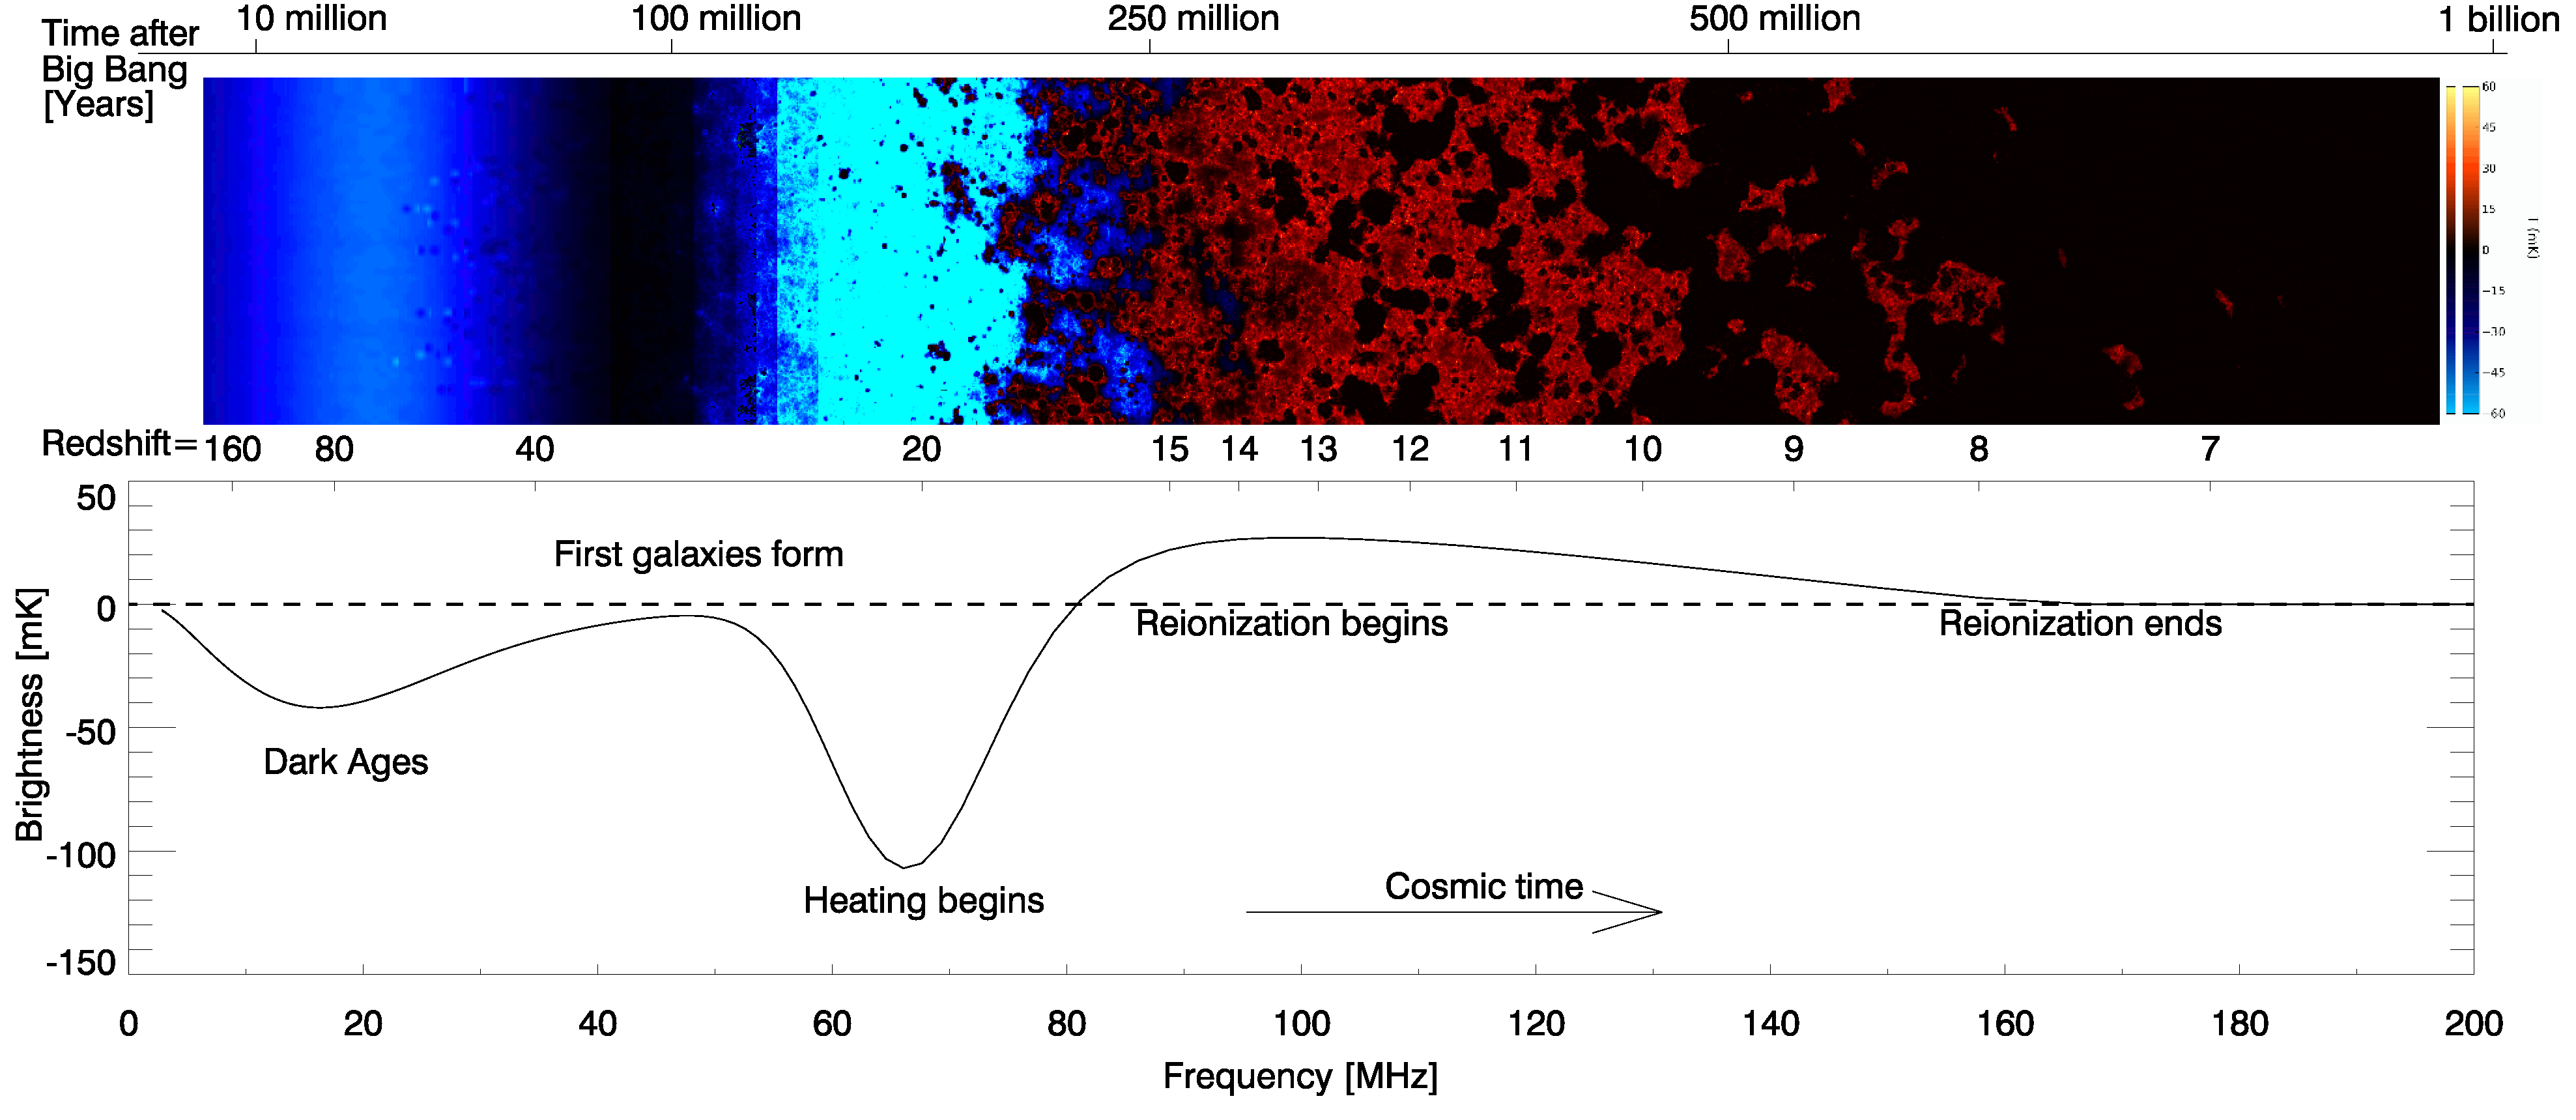
\includegraphics[width=\textwidth]{figures/chapter1/pritchard-2012-global-signal}
    \caption{
        Reproduced from \citet{2012RPPh...75h6901P}.
        get a license to use this figure (hit an error, but email sent (7-7-2018))
    }
    \label{fig:pritchard-global-signal}
\end{figure}

\begin{figure}[t]
    \centering
    \includegraphics[width=\textwidth]{figures/chapter1/history-of-the-universe/history-of-the-universe}
    \caption{
        A radial map of the universe. Known quasars are marked with circles and galaxies are marked
        with stars. The range of comoving distances probed by the OVRO-LWA and HERA are marked with a red
        rectangle and a blue rectangle respectively.
    }
    \label{fig:history-of-the-universe}
\end{figure}

For much of the universe's history, the intergalactic medium (IGM) is ionized or in radiative
equilibrium with the CMB.


\begin{equation}
    T_{21} \approx 27 \left[
        \overbrace{
            x_\text{HI} (1+\delta)
            \left(\frac{\Omega_b h}{0.0327}\right)
        }^{\text{quantity of HI}}
        \left(\frac{\Omega_m}{0.307}\right)^{-1/2}
        \left(\frac{1+z}{10}\right)^{1/2} \linebreak \times
        \overbrace{
            \left(\frac{T_\text{spin} - T_\text{CMB}(z)}{T_\text{spin}}\right)
        }^{\text{relative temperature}}
    \right] \, {\rm mK}
\end{equation}
\citep{2012RPPh...75h6901P}






Given knowledge of the
original wavelength of the photon, and the expansion history of the universe, we can calculate how
long the photon must have been in flight.


Today the CMB is a 2.7~K sea of photons that permeates the universe. This radiation is constantly
cooling due to the inexorable expansion of the universe.


Introduce low frequency telescopes.

Two different types of experiments are currently being designed to target the high-redshift 21~cm
transition:
\begin{enumerate}
    \item single antenna experiments that are attempting to measure the sky-averaged 21~cm signal,
        and
    \item large interferometers that are attempting to measure the three-dimensional spatial power
        spectrum of the 21~cm signal.
\end{enumerate}
Both types require exquisite calibration and roughly five orders of dynamic range against the
blindingly bright foreground radio emission, but are subject to different (but not exclusively
different) systematic instrumental errors.

\begin{figure}[t]
    \centering
    \includegraphics[width=\textwidth]{figures/chapter1/bowman-2018-absorption-trough}
    \caption{
        Reproduced from \citet{2018Natur.555...67B}.
        the Nature thing to get permission for this figure kept redirecting me to a blank page while
        I was trying to fill out the form. Why are all of these things garbage? Still, I need to get
        permission for this figure...
    }
    \label{fig:bowman-absorption-trough}
\end{figure}

\begin{figure}[t]
    \centering
    \includegraphics[width=\textwidth]{figures/chapter1/power-spectrum-upper-limits/power-spectrum-upper-limits}
    \caption{
        Power spectrum amplitude upper limits (95\% confidence) as a function of redshift. The
        shaded region denotes roughly where current theoretical predictions fall.
    }
    \label{fig:power-spectrum-upper-limits}
\end{figure}












\myputbib{thesis}
\end{bibunit}


\chapter{A Path Towards Calibration of the OVRO-LWA}
\label{chapter2}

\begin{bibunit}

\section{Design and Construction of the OVRO-LWA}

\begin{figure}
    \centering
    \includegraphics[width=\textwidth]{figures/chapter2/first-antenna}
    \caption{
        The first OVRO-LWA completed on 2013 March 8 with the class of Ay~122b (including the author
        of this thesis with the fractured ankle).
    }
    \label{fig:ovro-first-antenna}
\end{figure}

\begin{figure}[t]
    \centering
    \includegraphics[width=\textwidth]{figures/chapter2/lwa-antenna}
    \caption{
        Picture of an OVRO-LWA antenna.
    }
    \label{fig:ovro-lwa-pictures}
\end{figure}

\begin{figure}[t]
    \centering
    \includegraphics[width=\textwidth]{figures/chapter2/before-expansion}
    \caption{
        Snapshot image of the sky captured with the OVRO-LWA and using only the antennas located
        within the core of the array. The image covers the entire visible hemisphere in
        sine-projection.  A similar image constructed using the newer long-baseline antennas can be
        seen in Figure~\ref{fig:expansion-snapshot-image}.
    }
    \label{fig:core-snapshot-image}
\end{figure}

\begin{figure}[t]
    \centering
    \includegraphics[width=\textwidth]{figures/chapter2/after-expansion}
    \caption{
        Snapshot image of the sky captured with the OVRO-LWA and using the new long-baseline
        antennas. The image covers the entire visible hemisphere in sine-projection.  A similar
        image constructed using only the core of the interferometer can be seen in
        Figure~\ref{fig:core-snapshot-image}.
    }
    \label{fig:expansion-snapshot-image}
\end{figure}

The OVRO-LWA is a new low-frequency (27--85\,MHz instantaneous) radio interferometer constructed
during the course of this thesis and located near Big Pine, California. Construction began in 2013
with the first antenna completed in March of that year (see Figure~\ref{fig:ovro-first-antenna}).

The OVRO-LWA was initially composed of 256 antennas, with 251 of those antennas arranged within a
dense 200\,m diameter core in a configuration that is optimized for sidelobe levels in snapshot
imaging.  Each of these antennas consists of two crossed broadband dipoles with an active
balun/preamp, and the entire system is sky noise dominated over the range 20--80\,MHz
\citep{2012PASP..124.1090H}.  A picture of an OVRO-LWA antenna can be seen in
Figure~\ref{fig:ovro-lwa-pictures}. The primary beam of each OVRO-LWA antenna subtends a solid angle
of $\sim 8000\,\text{deg}^2$, with sensitivity to the entire visible hemisphere of the sky.

\todo{ARX boards}

The remaining five antennas are isolated from the core of the OVRO-LWA and equipped with radiometric
front ends as part of the LEDA experiment, which is attempting to measure the globally averaged
signal of \ion{H}{1} from the Cosmic Dawn \citep{2018MNRAS.478.4193P}.  The OVRO-LWA hosts the LEDA
correlator as its back-end, which is an FX correlator composed of 16 ROACH2 FPGAs that compose the F
stage, and 11 servers each with dual NVIDIA K20X GPUs that compose the X stage
\citep{2015JAI.....450003K}. This allows the correlator to perform full cross-correlation of 512
input signals with 58\,MHz instantaneous bandwidth.

During observations, data is streamed from the LEDA correlator to the All-Sky Transient Monitor
(ASTM), which houses the compute nodes used for post-processing and imaging.  The ASTM is composed
of 10 identical nodes each with a 16-core Intel Xeon E5-2630 v3 CPU and 64\,GB of memory. Five
additional servers provide 565\,TB of storage capacity through the Lustre high performance file
system.

The initial 256 antenna interferometer was therefore capable of imaging the entire visible
hemisphere in snapshot images with 1$\arcdeg$ angular resolution. An example snapshot image can be
seen in Figure~\ref{fig:core-snapshot-image}.  In 2015, an additional 32 antennas were installed
that extended the maximum baseline of the interferometer to 1.5\,km and improved the angular
resolution to 8$\arcmin$. This improved angular resolution can be seen in
Figure~\ref{fig:expansion-snapshot-image}. In a final future stage of development, an additional 64
antennas will be installed that extend the maximum baseline to 2.6\,km, which will see improved
$uv$-coverage at long baselines and improved $5\arcmin$ angular resolution.

While this thesis focuses on the use of the OVRO-LWA to detect the high-redshift signature of
neutral hydrogen from the Cosmic Dawn, the OVRO-LWA facilitates a diverse set of scientific
motivations including the study of stellar and planetary magnetospheres, radio follow-up of gamma
ray bursts \citep{2017arXiv171106665A} and neutron star mergers, solar dynamic imaging spectroscopy,
and the detection of high energy cosmic rays \citep{caltechthesis11016}.

With the exception of detecting high energy cosmic rays---which uses a custom firmware and
processing pipeline that cannot operate in parallel with ordinary correlation---there are two
complementary software pipelines that service the scientific goals of the OVRO-LWA:
\begin{enumerate}
    \item A widefield snapshot imaging pipeline that images the entire visible hemisphere every
        13\,s using WSCLEAN \citep{2014MNRAS.444..606O}.
    \item A novel approach specialized for drift-scanning interferometers that can image the entire
        sky (above a limiting declination) in a single synthesis imaging step.
\end{enumerate}
This chapter will describe the calibration, source removal routines purpose built for the OVRO-LWA
and used by both pipelines. Additionally, in \S\ref{sec:commissioning-challenges} I will discuss
some of the challenges involved with commissioning the OVRO-LWA that have been overcome to bring the
OVRO-LWA into existence, to first light, and finally its first scientific results.  Finally, the
latter pipeline will be discussed in considerable depth in Chapters~\ref{chapter3} and
\ref{chapter4}.

\section{Calibration of a Low-Frequency Interferometer}

Gain calibration amounts to determining the optimal set of Jones matrices $G_i$ for each antenna $i$
such that
\begin{align}
    \b V_{ij, \text{measured}} &= \b G_i \, \b V_{ij, \text{model}} \, \b G_j^*
        + \b N_{ij} \\
    \begin{pmatrix}
        V_{ij, \text{measured}}^{xx} & V_{ij, \text{measured}}^{xy} \\
        V_{ij, \text{measured}}^{yx} & V_{ij, \text{measured}}^{yy} \\
    \end{pmatrix} &=
    \begin{pmatrix}
        g_{i}^{xx} & g_{i}^{xy} \\
        g_{i}^{yx} & g_{i}^{yy} \\
    \end{pmatrix}
    \begin{pmatrix}
        V_{ij, \text{model}}^{xx} & V_{ij, \text{model}}^{xy} \\
        V_{ij, \text{model}}^{yx} & V_{ij, \text{model}}^{yy} \\
    \end{pmatrix}
    \begin{pmatrix}
        g_{j}^{xx} & g_{j}^{xy} \\
        g_{j}^{yx} & g_{j}^{yy} \\
    \end{pmatrix}^* +
    \begin{pmatrix}
        n_{j}^{xx} & n_{j}^{xy} \\
        n_{j}^{yx} & n_{j}^{yy} \\
    \end{pmatrix}\,,
\end{align}
where $\b V_{ij,\text{measured}}$ is the Jones matrix of measured visibilities on the baseline
$i-j$, $\b V_{ij,\text{model}}$ is the Jones matrix of model visibilities (i.e., ideally what would
have been measured if the antenna and receiver did not impart any additional gain or phase), and $\b
N_{ij}$ is additional noise.

A typical calibration strategy using the Very Large Array (VLA) involves periodically pointing at a
known compact point source. For a compact point source at the phase center, the phase of all
visibilities should be zero, and the amplitude is given by the known flux (and if necessary, the
polarization) of the source.

The OVRO-LWA is capable of imaging the entire hemisphere in a snapshot image. This brings its own
unique calibration challenges because it is currently impossible to isolate a single compact point source
within the field of view of the interferometer.\footnote{
    Gated pulsar observations could, in principle, achieve this isolation. This capability is a key
    development area for the OVRO-LWA.
}
Due to the wide field of view, determining an accurate gain calibration relies on a detailed sky
and antenna beam model. Mistakes or omissions in the sky model can, for example, generate artificial
ripples in the bandpass calibration that will impact the interferometer's ability to cleanly
separate foreground emission from cosmological 21~cm emission \citep{2016MNRAS.461.3135B}.

Furthermore, at frequencies $\nu < 100\,\text{MHz}$ there are few flux calibrators.
\citet{1977A&A....61...99B} determined the absolute spectrum of Cyg~A between 20~MHz and 2~GHz.
\citet{2012MNRAS.423L..30S} added six additional calibrators, and \citet{2017ApJS..230....7P} used
the VLA 4-band system to bring the total number of available calibrators to 11. However, in
\S\ref{sec:flux-scale} I will show that the latter spectra can diverge rapidly from truth below
50~MHz.

Detailed sky and beam models are therefore generally an important calibration requirement for
low-frequency interferometers. In \S\ref{chapter3}, I derived an empirical beam model for the
OVRO-LWA and developed a new imaging formalism that captures the entire visible sky in a single
synthesis imaging step that can be used as part of a self-calibration loop.

The calibration routine itself is adapted from a variant of alternating least-squares developed by
\citet{2008ISTSP...2..707M} and \citet{2014A&A...571A..97S}. At each step this algorithm seeks to
minimize
\begin{equation}\label{eq:stefcal-step}
    \b G_i = \argmin \sum_{j \neq i}
        \left\|
            \b V_{ij, \text{measured}} - \b G_i \, \b V_{ij, \text{model}} \, \b G_j^*
        \right\|^2\,
\end{equation}
where each of the elements of $\b G_j^*$ are considered fixed. Equation~\ref{eq:stefcal-step} is
therefore a linear least-squares optimization and can be rapidly solved. However, by fixing $\b
G_j^*$ these iterations tend to oscillate about a minimum of $\chi^2$. These oscillations can be
damped by averaging subsequent iterations, and \citet{2014A&A...571A..97S} demonstrated that this
simple gradient-free optimization strategy converges remarkably quickly.

Some interferometers (e.g., HERA and the MWA), recognizing the difficulty of gain calibration at low
frequencies, have opted for partly redundant antenna configurations. These configurations can solve
for many of their calibration parameters internally without relying on an incomplete sky model and
potentially inaccurate antenna beam model \citep{2010MNRAS.408.1029L}. However, these
interferometers sacrifice imaging fidelity, which is useful for establishing the remaining
calibration parameters (e.g., the overall bandpass cannot be solved for in an internal
redundant-calibration routine).\footnote{
    The HERA collaboration is currently investigating the possibility of determining the overall
    bandpass through redundancies between frequency channels. The author of this thesis is not
    optimistic about this approach.
}

\section{Source Removal and Direction-Dependent Calibration}

Because the OVRO-LWA antenna layout is optimized for sidelobe levels in snapshot imaging, the
point-spread function (PSF) is pretty good.

\section{Commissioning Challenges}
\label{sec:commissioning-challenges}

\subsection{Computing Antenna Positions}

\begin{figure}
    \centering
    \includegraphics[width=\textwidth]{figures/chapter2/northing-easting-mistake/northing-easting-mistake}
    \caption{
        Illustration of the error in the WCS prior to a correction to the antenna positions. The
        image is a difference between an image constructed with the incorrect antenna positions and
        the corrected antenna positions. The arrow denotes the direction and approximate center of
        the rotation.
    }
    \label{fig:northing-easting-mistake}
\end{figure}

Early images produced by the OVRO-LWA (prior to 2015 October 16) were afflicted by an apparent
rotation in the World Coordinate System (WCS).

\subsection{RFI Localization}

\begin{figure}
    \centering
    \begin{tabular}{cc}
        \includegraphics[width=0.45\textwidth]{figures/chapter2/google-maps-rfi-localization} &
        \includegraphics[width=0.45\textwidth]{figures/chapter2/power-line-picture} \\
        (a) & (b) \\
    \end{tabular}
    \caption{
        (a) The localization region for a source of RFI south of the OVRO-LWA and near the town of
        Big Pine. Satellite imagery \textcopyright2018 Google. Map data \textcopyright2018 Google.
        (b) Image of a high-voltage power line overlooking OVRO near the localization region.
    }
    \label{fig:rfi-localization}
\end{figure}

An ongoing challenge faced by the OVRO-LWA is the presence of broadband sources of RFI in the
vicinity of the observatory. Due to the entire-hemisphere field of view of the OVRO-LWA, these
sources appear as points on the horizon that limit the sensitivity of snapshot images through
additional sidelobe noise. Fortunately, because these sources are typically in the near-field of the
interferometer, the curvature of the incoming wavefront can be used to infer the distance to each
source of RFI.

The path difference from a source in the near-field of an interferometer located at the position
$(\xi, \eta, \zeta)$ to two antennas located respectively at $(x_i, y_i, z_i)$ and $(x_j, y_j, z_j)$
is
\begin{equation}\label{eq:nearfield-path-difference}
    \Delta l^\text{near-field}_{ij} =
        \sqrt{(x_j - \xi)^2 + (y_j - \eta)^2 + (z_j - \zeta)^2}
        - \sqrt{(x_i - \xi)^2 + (y_i - \eta)^2 + (z_i - \zeta)^2}\,.
\end{equation}
In the limit that the distance of the source goes to infinity, we recover the familiar expression
\begin{equation}\label{eq:farfield-path-difference}
    \Delta l^\text{far-field}_{ij} = \frac{1}{D}\Big(
        (x_i - x_j)\,\xi + (y_i - y_j)\,\eta + (z_i - z_j)\,\zeta
    \Big)\,,
\end{equation}
where $D$ is the distance to the source. The correlation measured between two antennas for a source
in the near-field of the interferometer is therefore
\begin{equation}\label{eq:nearfield-visibilities}
    V_{ij} = F \exp\left(2\pi i \frac{\Delta l^\text{near-field}_{ij}}{\lambda}\right)\,,
\end{equation}
where $V_{ij}$ is the visibility measured between antennas $i$ and $j$, $F$ is the apparent
brightness of the source, and $\lambda$ is the wavelength. Equation~\ref{eq:nearfield-visibilities}
can then be used to fit for the position of a source including its distance.

In order to improve sensitivity to these RFI sources,



\myputbib{thesis}
\end{bibunit}


\chapter{The Radio Sky at Meter Wavelengths: $m$-mode Analysis Imaging with the OVRO-LWA}



\chapter{21 cm Cosmology of the Cosmic Dawn: First Spatial Power Spectrum Limits with the OVRO-LWA}



\chapter{Conclusion}
\label{chapter5}

In this thesis I have described the construction and commissioning of the OVRO-LWA.

Construction of the OVRO-LWA

As part of the commissioning of the OVRO-LWA, I developed several tools that have allowed the
instrument to capture high-dynamic range, high-fidelity images.

I wrote \texttt{TTCal}

In Chapter~\ref{chapter3}, I described the development and demonstration of a new widefield imaging
technique specialized for drift-scanning interferometers like the OVRO-LWA.

Foreground mitigation and instrumental calibration are the limiting factors in essentially all
attempts to measure the spatial power spectrum of 21\,cm fluctuations from the EoR and Cosmic Dawn.

In Chapter~\ref{chapter4}, I placed the deepest limits to date on the amplitude of 21\,cm
fluctuations from the Cosmic Dawn, and the first limits at $z > 18$.

This measurement was the first demonstration of the double KL transform foreground filter on a real
measured dataset. I showed that while this filter can help to mitigate foreground contamination, it
is not a replacement for careful calibration. Calibration and modeling errors can allow foreground
emission to leak through the foreground filter.

This measurement, however, was limited by systematic errors.

Future requirements and directions

Better calibration

Better peeling

Beam mapping



%\appendix
%\chapter{Open-Source Software}

\section{TTCal}

\section{BPJSpec}

\section{CasaCore.jl}

\section{LibHealpix.jl}

\section{UnitfulAstro.jl}




\end{document}

